\chapter{Optimization of continuum structures}
In the previous chapter, we learned how to transform a continuous elastic problem defined on a two-dimensional domain into a discrete problem using finite elements. Now we want to optimize such problems.

\begin{objectives}{}{objectives_continuum}
After studying this chapter and finishing the exercise, you should be able to 
\begin{itemize}[label=$\dots$]
    \item transfer solution methods from intrinsically discrete truss structures to FEM-discretized problems
    \item explain the solution process for variable thickness sheets (size optimization) 
    \item solve for binary topologies using the SIMP approach
    \item discuss numerical problems in topology optimization
    \item apply filters to deal with numerical problems and manufacturing constraints in topology optimization
    \item explain the need for mesh morphing in shape optimization
\end{itemize}
\end{objectives}

\section{Size optimization}
\label{sec:variable_thickness_sheet}
Let's consider a two-dimensional domain discretized with finite elements, in which we can adjust the thickness of each element. We may seek the best distribution of thicknesses $\mathbf{d}$ to minimize compliance $C$ with a constrained amount of material volume $V_0$. This problem can be formulated in analogy to the standard problem of sizing optimization stated in Equation \eqref{eq:size_optimization}

\begin{equation}
    \begin{aligned}
        \min_{\mathbf{d}} \quad & C(\mathbf{d}) = \mathbf{f} \cdot \mathbf{u}(\mathbf{d})\\
        \textrm{s.t.} \quad & \mathbf{d} \cdot \mathbf{A} - V_0 \le 0  \\
                            & \mathbf{d} \in \mathcal{D}\\
    \end{aligned}
    \label{eq:sheet_optimization}
\end{equation}
where $\mathbf{A}$ denotes the area of an element. Mathematically, this problem is equivalent to the truss problem and can be solved in the same way: We formulate the Lagrangian
\begin{equation}
    \mathcal{L}(\mathbf{d}, \mu) = C(\mathbf{d}) + \mu \left( \mathbf{d} \cdot \mathbf{A} - V_0 \right) 
    \label{eq:lagrangian_sheet_optimization}
\end{equation}
and determine its derivative
\begin{equation}
    \frac{\partial \mathcal{L} (\mathbf{d}, \mu)}{\partial d_j} 
    = \frac{\partial C(\mathbf{d})}{\partial d_j} + \mu A_j 
\end{equation}
with 
\begin{equation}
    \frac{\partial C}{\partial d_j} = - \mathbf{u}_j(\mathbf{d})  \cdot \mathbf{k}^0_j \cdot \mathbf{u}_j(\mathbf{d}) = -2w_j(\mathbf{d}).
    \label{eq:sensitivity_sheet}
\end{equation}
In comparison to Equation \eqref{eq:compliance_sensitivity} for trusses with four degrees of freedom, the element displacement vector contains eight degrees of freedom for these 2D problems with linear quad elements ($\mathbf{u}_j \in \mathcal{R}^8, \mathbf{k}^0_j \in \mathcal{R}^{8\times 8}$). 

Just like the truss problem, the variable thickness sheet problem can be approximated using MMA with lower asymptotes only. Subsequently, it is solved with the dual method and a line search to find the Lagrange parameter $\mu$. The entire procedure is identical to Section \ref{sec:truss_topology}, if we replace the truss cross sections $\mathbf{a}$ with element thicknesses $\mathbf{d}$ and the truss lengths $\mathbf{l}$ with element areas $\mathbf{A}$.

\begin{example}{Size optimization with MMA}{cantileveroptimizationexample}
    Consider a FEM cantilever beam from the previous example. Instead of just computing the displacements, we are now interested in finding the optimal thickness of each element given a volume constraint.

    We formulate the following algorithm to solve that problem: 
    \begin{enumerate}
        \item Define the cantilever FEM model with all nodes $\mathcal{N}$, elements $\mathcal{E}$, material property $E$, volume constraint $V_0$, design limits $\mathbf{d}^l, \mathbf{d}^u$ and the initial design choice $\mathbf{d}^0$.
        \item Compute the displacements $\mathbf{u}^k = \mathbf{u}(\mathbf{d}^k)$ by solving the FEM system for the current design $\mathbf{d}^k$.
        \item Compute the strain energies densities for all elements using the previously computed displacements   
        \begin{equation}
            w^k_j(\mathbf{d}^k) = \frac{1}{2}\mathbf{u}^k_j  \cdot \mathbf{k}^0_j \cdot \mathbf{u}^k_j
        \end{equation}
        \item Compute the lower asymptotes as $\mathbf{L}^k =\mathbf{d}^k - s (\mathbf{d}^u - \mathbf{d}^l)$ with $s \in (0,1)$ during the first two iterations and according to 
        \begin{equation}
            L^k_j = 
            \begin{cases}
                d^k_j - s  (d^{k-1}_j-L^{k-1}_j) & (d_j^k-d_j^{k-1})(d_j^{k-1}-d_j^{k-2}) < 0\\
                d^k_j - \frac{1}{\sqrt{s}}  (d^{k-1}_j-L^{k-1}_j) & \text{else}
            \end{cases}
        \end{equation}
        in the following iterations.
        \item Compute the lower move limit as 
        \begin{equation}
            \tilde{\mathbf{d}}^{l,k} = \max(\mathbf{d}_l,  0.9 \mathbf{L}^k + 0.1 \mathbf{d}^k)
        \end{equation}
        \item Evaluate the analytical solution
            \begin{align}
                \hat{d}_j(\mu) &= L_j^k + \sqrt{\frac{2 w_j (\mathbf{d}^k)
                (L^k_j-d^k_j)^2}{\mu A_j}} \\
                \mathbf{d}^* (\mu) &= \max\left(\tilde{\mathbf{d}}^{l,k}, \min \left(\hat{\mathbf{d}}(\mu), \mathbf{d}_u \right)\right)
            \end{align}
        \item Perform a line search to find the root $\mu^*>0$ in 
        \begin{equation}
            \frac{\partial \underline{\mathcal{L}}}{\partial \mu}(\mu) = \mathbf{A} \cdot \mathbf{d}^* (\mu) - V_0  = 0
        \end{equation}
        with Newton's method or bisection method. 
        \item Repeat with steps 2-7 until convergence or a maximum number of iterations is reached.
    \end{enumerate}

    The following image shows a result of the algorithm for the cantilever problem stated above. Black areas use the full maximum thickness $\mathbf{d}^u$ and white areas use the minimum thickness $\mathbf{d}^l$. The intermediate values are represented by different shades of gray.

    \begin{center}
        \includesvg[width=\linewidth]{figures/cantilever_fem_optimized.svg}
    \end{center}
    
\end{example}

\section{Topology optimization with MMA}
In a topology optimization of continuum structures, we want to optimize the neighborhood relations of a structure. While the size or shape of an object could be changed by some deformation, we cannot change a topology to another by a "rubber-like" deformation. Essentially this means, in topoplogy optimization we are seeking the fundamental structure of a component: Which parts are connected? How many holes are in it? 

\begin{example}{Topology of steering wheels}{steeringwheelexample}
    Out of the following schematic steering wheels, the top left wheel may be transformed to the bottom center wheel by an appropriate deformation. They have the same topology, but different shapes. However, they cannot be transformed to any other steering wheel, as this would require formation of new holes and break the neighborhood relations. 
    \begin{center}
        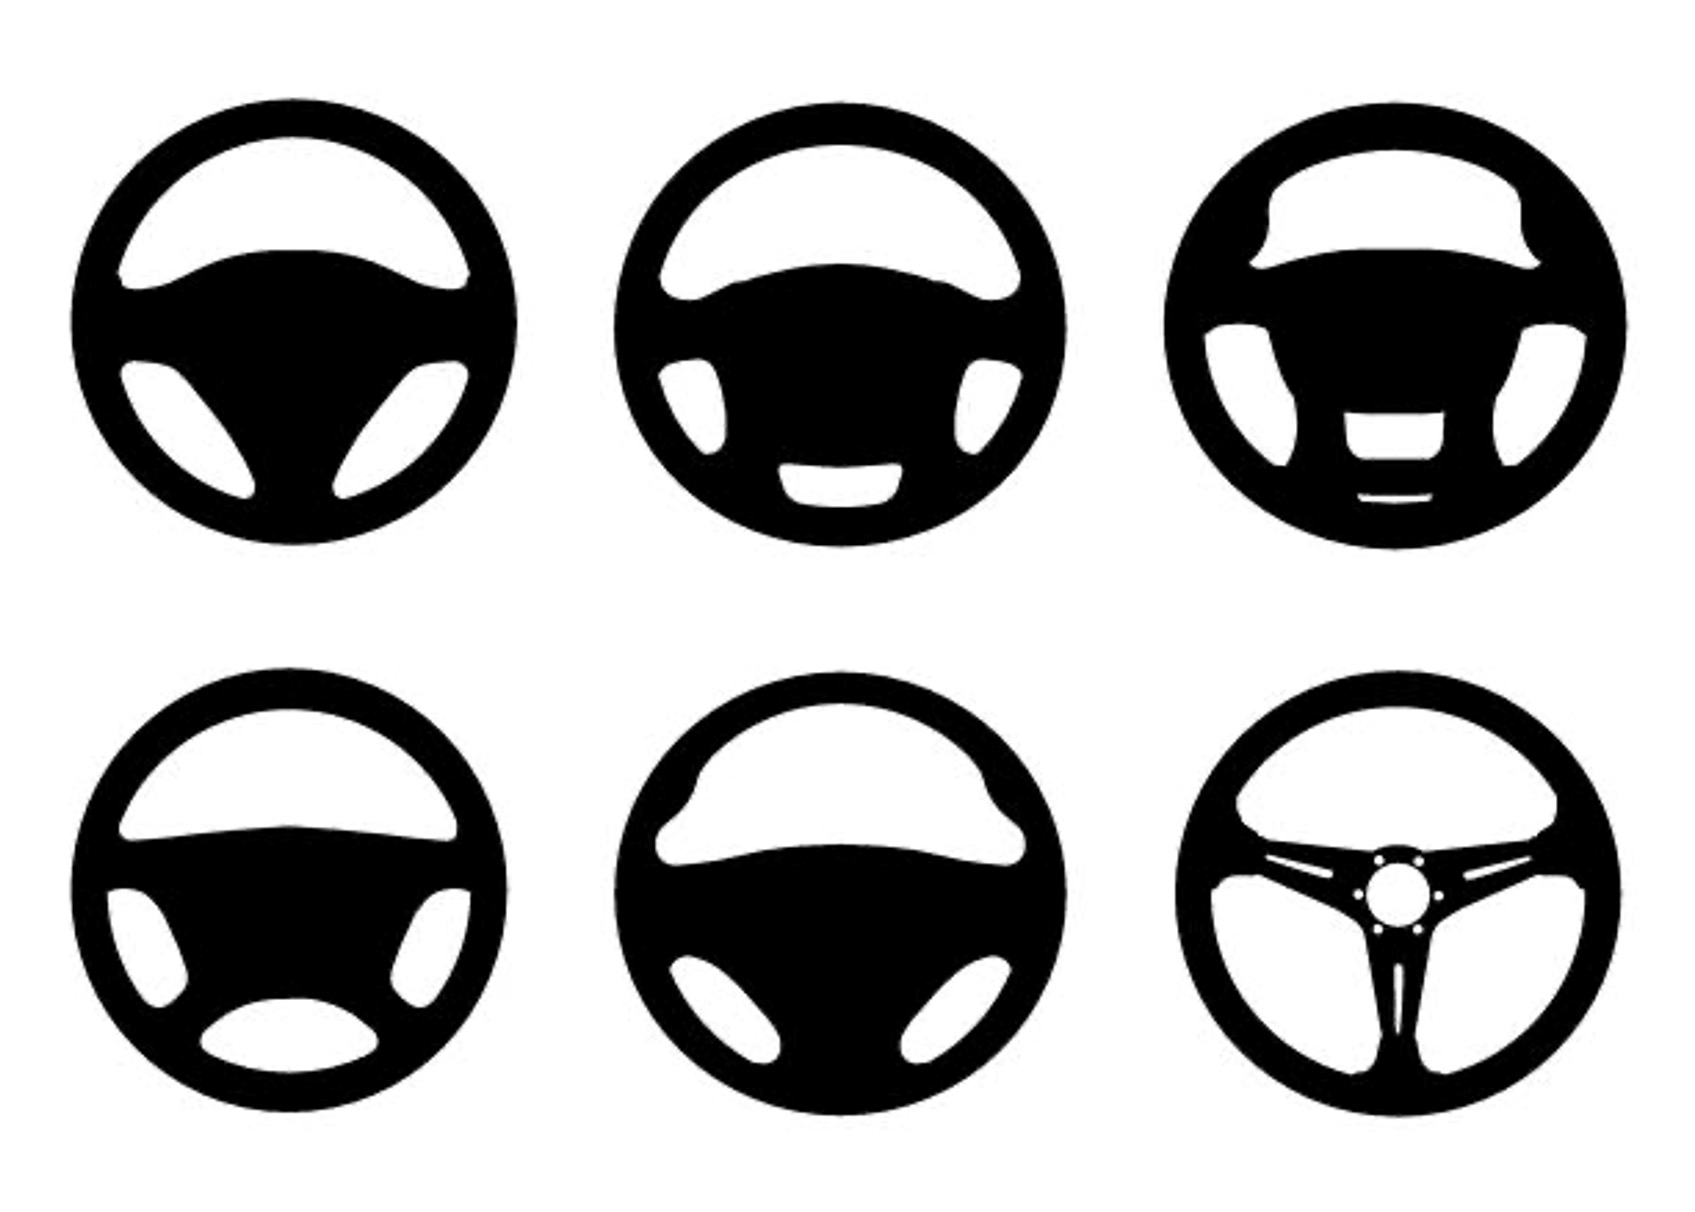
\includegraphics[width=0.8\textwidth]{figures/steeringwheels.png}
    \end{center}
\end{example}

There are two main approaches to optimize the topology \cite{Eschenauer2001}: In a \emph{geometry-based} formulation, we describe the domain in a dynamic fashion ( e.g. by a Level-Set method) and modify this geometry towards the optimum (e.g. by empirical growth rules like SKO or CAIO).
In a \emph{material-based} formulation, we describe the entire domain with finite elements and then seek a material distribution where each element is either completely filled or completely unfilled with material. In this lecture, we focus entirely on the latter approach.

We can formulate such a problem by reinterpreting the thickness variable as a normalized material density $\pmb{\rho}$, where $\rho_j=1$ indicates presence of material and $\rho_j=0$ indicates absence of material in element $j$. The stiffness of each element becomes a function of $\rho_j$, e.g. 
\begin{equation}
    \mathbb{C}(\rho_j)=
    \begin{cases}
        \mathbb{C} & \text{if} \quad \rho_j = 1 \\
        0          & \text{if} \quad \rho_j = 0
    \end{cases}
\end{equation}

Then, the problem statement reads
\begin{equation}
    \begin{aligned}
        \min_{\pmb{\rho}} \quad & C(\pmb{\rho}) = \mathbf{f} \cdot \mathbf{u}(\pmb{\rho})\\
        \textrm{s.t.} \quad & \pmb{\rho} \cdot \mathbf{V} - V_0 \le 0  \\
                            & \rho_j \in \{0, 1\}\\
    \end{aligned}
    \label{eq:topology_optimization}
\end{equation}

where the only change compared to Equation \eqref{eq:sheet_optimization} is the discrete nature of the design variables $\pmb{\rho}$ and the name of the design variables. 


As mentioned during truss optimization, the binary problem is notoriously hard to solve. Hence we use \emph{Solid Isotropic Material with Penalization} (SIMP) again, which is denoted as 
\begin{equation}
    \mathbb{C}(\rho_j)= \rho_j^p \mathbb{C}
\end{equation}
for the generalized FEM problem. 

Incorporating the SIMP method to the optimization is straight-forward: The element stiffness for a 2D problem with element thicknesses $d_j$ is now 
\begin{equation}
    \mathbf{k}_j(\rho_j) =  \rho_j^p d_j \mathbf{k}^0_j
\end{equation}
and consequently, the gradient becomes 
\begin{equation}
    \frac{\partial\mathbf{k}_j(\rho_j)}{\partial \rho_j} =  p \rho_j^{p-1}  d_j\mathbf{k}^0_j.
\end{equation}
Then, we just need to adjust the sensitivity (see Equation \ref{eq:sensitivity_sheet}) slightly towards
\begin{equation}
    \frac{\partial C}{\partial \rho_j} (\pmb{\rho}) = - p \rho_j^{p-1} d_j\mathbf{u}_j(\pmb{\rho})  \cdot \mathbf{k}^0_j \cdot \mathbf{u}_j(\pmb{\rho}) = -2 p \rho_j^{p-1} d_j w_j(\pmb{\rho}).
    \label{eq:sensitivity_topology}
\end{equation}

\begin{example}{Topology optimization with MMA and SIMP}{cantileversimpoptimizationexample}
    Consider the FEM cantilever beam from the previous example. We slightly change the algorithm towards the following:  
    \begin{enumerate}
        \item Define the cantilever FEM model with all nodes $\mathcal{N}$, elements $\mathcal{E}$, material property $E$, volume constraint $V_0$, a lower design limit $\pmb{\rho}^l$ and the initial design choice $\pmb{\rho}^0$.
        \item Compute the displacements $\mathbf{u}^k = \mathbf{u}(\pmb{\rho}^k)$ by solving the FEM system for the current design $\pmb{\rho}^k$.
        \item Compute the strain energies densities for all elements using the previously computed displacements   
        \begin{equation}
            w^k_j(\pmb{\rho}^k) = \frac{1}{2}\mathbf{u}^k_j \cdot \mathbf{k}^0_j \cdot \mathbf{u}^k_j
        \end{equation}
        \item Compute the lower asymptotes as $\mathbf{L}^k =\pmb{\rho}^k - s (\mathbf{1} - \pmb{\rho}^l)$ with $s \in (0,1)$ during the first two iterations and according to 
        \begin{equation}
            L^k_j = 
            \begin{cases}
                \rho^k_j - s  (\rho^{k-1}_j-L^{k-1}_j) & (\rho_j^k-\rho_j^{k-1})(\rho_j^{k-1}-\rho_j^{k-2}) < 0\\
                \rho^k_j - \frac{1}{\sqrt{s}}  (\rho^{k-1}_j-L^{k-1}_j) & \text{else}
            \end{cases}
        \end{equation}
        in the following iterations.
        \item Compute the lower move limit as 
        \begin{equation}
            \tilde{\pmb{\rho}}^{l,k} = \max(\pmb{\rho}_l,  0.9 \mathbf{L}^k + 0.1 \pmb{\rho}^k)
        \end{equation}
        \item Evaluate the analytical solution
            \begin{align}
                \hat{\rho}_j(\mu) &= L_j^k + \sqrt{\frac{2 p \rho_j^{p-1} d_j w_j (\pmb{\rho}^k)
                (L^k_j-d^k_j)^2}{\mu V_j}} \\
                \pmb{\rho}^* (\mu) &= \max\left(\tilde{\pmb{\rho}}^{l,k}, \min \left(\hat{\pmb{\rho}}(\mu), \mathbf{1} \right)\right)
            \end{align}
        \item Perform a line search to find the root $\mu^*>0$ in 
        \begin{equation}
            \frac{\partial \underline{\mathcal{L}}}{\partial \mu}(\mu) = \mathbf{V} \cdot \pmb{\rho}^* (\mu) - V_0  = 0
        \end{equation}
        with Newton's method or bisection method. 
        \item Repeat with steps 2-7 until convergence or a maximum number of iterations is reached.
    \end{enumerate}

    This procedure results in the following solution:
    \begin{center}
        \includesvg[width=0.7\linewidth]{figures/cantilever_fem_optimized_binary.svg}
    \end{center}
\end{example}

Obviously, the SIMP approach helps us to find a binary solution of the discretized problem stated in Equation \eqref{eq:topology_optimization}. However, we may ask ourselves if there is a unique solution to this problem independent of discretization. And it turns out, the answer is no: You can improve any given design by replacing it with finer structures in a process that goes on indefinitely \cite{Christensen2008}. 
In addition to the theoretical non-existence of a solution, this also means that our solution is \emph{mesh-dependent}: If we want to refine the solution, we may end up with a totally different solution. 

Even if we were to accept mesh dependence and the theoretical problem of ill-posedness, we are still left with challenges in the resulting designs. First of all, fine structures may be hard to manufacture. Even additive manufacturing methods are limited to some minimal structure size. Secondly, we may observe checkerboard-like patterns on the structure. These are numerical artifacts from the fact that we use linear shape functions which lead to an overestimation of the stiffness for that configuration.

\begin{example}{Mesh dependency}{cantileverdiscoptimizationexample}
    We can increase the resolution of the previous examples to achieve better compliance results. However, this demonstrates the mesh-dependence of the solution as we observe different structures in both cases. Additionally, the resulting fine structures might be difficult to manufacture.
    \begin{center}
        \includesvg[width=0.7\linewidth]{figures/cantilever_fem_optimized_binary_fine.svg}
        \includesvg[width=0.7\linewidth]{figures/cantilever_fem_optimized_binary_extra_fine.svg}
    \end{center}
\end{example}

We can address all these problems with the introduction of filters as a regularization \cite{Harzheim2014, Lazarov2011}. There are two traditional approaches for mesh-independent filtering: \emph{density filtering} and \emph{sensitivity filtering}. In density filtering, we replace the density $\pmb{\rho}$ with a weighted sum of neighboring densities, and use this filtered density $\tilde{\pmb{\rho}}$ in the stiffness evaluation
\begin{equation}
    \mathbb{C}(\rho_j)= \tilde{\rho}_j^p \mathbb{C}.
\end{equation}
The filtered density is computed according to 
\begin{equation}
    \tilde{\rho}_j (\pmb{\rho}) = \frac{\sum_i H_{ji} A_i \rho_i}{\sum_i H_{ji} A_i}
\end{equation}
with a distance weighting matrix
\begin{equation}
    H_{ji} = 
    \begin{cases}
        R-\textrm{dist}(i,j) & \text{if} \quad \textrm{dist}(i,j) \le R \\
        0 & \text{else},
    \end{cases}
\end{equation}
where $R$ describes the filter radius and $\textrm{dist}(i,j)$ the distance between element centers of elements $i$ and $j$. This filter results in a structural weakening of structures finer than $R$, as they get smeared with neighboring empty elements. Hence, the filter solves the mesh-dependency problem, prevents structures that cannot be manufactured and prevents checkerboard patterns. However, we need to account for the filter during sensitivity computation by 
\begin{equation}
    \frac{\partial C}{\partial \rho_j} 
    = \frac{\partial C}{\partial \tilde{\rho}_m} \frac{\partial \tilde{\rho}_m}{\partial \rho_j}
    = \frac{\partial C}{\partial \tilde{\rho}_m}  \frac{H_{jm} A_m }{\sum_i H_{ji} A_i}
\end{equation}
and in the volume constraint.

An alternative to filtering densities is filtering of sensitivities. We may compute the filtered sensitivity as
\begin{equation}
    \widetilde{\frac{\partial C}{\partial \rho_j}} = \frac{1}{\rho_j} \frac{\sum_i H_{ji} A_i \rho_i \frac{\partial C}{\partial \rho_i} }{\sum_i H_{ji} A_i}
\end{equation}
which is a purely heuristic concept, i.e. there is no mathematical proof for this filter to work \cite{Sigmund1998}. However, we can implement this formulation simply by replacing the sensitivities in \eqref{eq:sensitivity_topology} with filtered sensitivities. This is very efficient, simple to implement and experience shows that this filter works quite well.

\begin{example}{Sensitivity filtering}{cantileverfilterexample}
    The following images show the optimized cantilever beams from previous examples with enabled sensitivity filtering employing the same filtering radius for each resolution. Filtering prevents small structures and regularizes the problem such that we achieve the same optimal designs for different mesh sizes.
    \begin{center}
        \includesvg[width=0.7\linewidth]{figures/cantilever_fem_optimized_binary_filtered.svg}
        \includesvg[width=0.7\linewidth]{figures/cantilever_fem_optimized_binary_fine_filtered.svg}
        \includesvg[width=0.7\linewidth]{figures/cantilever_fem_optimized_binary_extra_fine_filtered.svg}
    \end{center}
\end{example}

There is one more challenge in the SIMP formulation of the standard topology optimization problem: For $p>1$, the problem is not convex anymore and different starting points may result in different local minima \cite{Christensen2008}. A strategy to cure termination at non-global minima is a gradual increase of $p$ starting from $p=1$ or using multiple starting points.

\section{Topology optimization with optimality criteria}
The solution via MMA is in line with the previous chapters of this manuscript and is able to solve arbitrary problems beyond the compliance minimization stated in problem \eqref{eq:topology_optimization}. Historically, this specific problem was first solved with the \emph{optimality criteria method} instead of convex approximations. The idea here is that we can use the gradient of the Lagrangian
\begin{equation}
    \mathcal{L}(\pmb{\rho}, \mu) = C(\pmb{\rho}) + \mu \left( \pmb{\rho} \cdot \mathbf{V} - V_0 \right),
\end{equation}
which is
\begin{equation}
    \frac{\partial \mathcal{L} (\pmb{\rho}, \mu)}{\partial\rho_j} 
    = \frac{\partial C(\pmb{\rho})}{\partial \rho_j} + \mu V_j = 0,
\end{equation}
at the optimal point, to formulate an optimality condition
\begin{equation}
    G_j = \frac{-\frac{\partial C(\pmb{\rho})}{\partial \rho_j}}{\mu V_j} = \frac{p \rho_j^{p-1} d_j \mathbf{u}_j(\pmb{\rho})  \cdot \mathbf{k}^0_j \cdot \mathbf{u}_j(\pmb{\rho})}{\mu V_j} = 1
\end{equation}
that must be fulfilled at the optimum whenever a variable does not reach its bounds.
A heuristic algorithm can now compute $G_j$ and adjust $\rho_j$ such that $G_j$ approaches 1. We may realize that increasing $\rho_j$ increases the stiffness and hence decreases the displacement for a given load. Consequently, increasing $\rho_j$ decreases $G_j$ and vice versa. Hence, an update rule 
\begin{equation}
    \hat{\rho}_j^{k+1} = \left(G_j^k\right)^\xi \rho_j^k 
\end{equation}
drives the solution towards the optimal point $\rho_j^*$, where $G^*_j=1$. The exponent $\xi \in (0,1]$ stabilizes the algorithm with typical values being $\xi=0.5$ \cite{Harzheim2014}. 

In addition, we employ move limits 
\begin{align}
    \rho_j^{l,k} &= \max \left(\rho_j^l, (1-m)\rho_j^k \right) \\
    \rho_j^{u,k} &= \min \left(\rho_j^u, (1+m)\rho_j^k \right)
\end{align}
to compute the next value as 
\begin{equation}
    \rho_j^{k+1} = \max \left( \min \left(\hat{\rho}_j^{k+1}, \rho_j^{u,k} \right), \rho_j^{l,k} \right).
\end{equation}
The move limits reduce the maximum step width and account for bounds on the design variables. 

To compute $G_j$, we need to determine the value of the Lagrange multiplier $\mu$. For the compliance problem, we can intuitively assume that the stiffest structure will use all material and consequently, that the volume constraint will be active. The Lagrange multiplier may be found with the bisection method on the feasibility condition
\begin{equation}
    \frac{\partial \mathcal{L}}{\partial \mu} = \pmb{\rho}(\mu) \cdot \mathbf{V} - V_0 = 0.
\end{equation}

\begin{example}{Algorithm with optimality criteria}{ocexample}
    Consider a FEM cantilever beam from the previous example. 

    We formulate the following algorithm to solve that problem: 
    \begin{enumerate}
        \item Define the cantilever FEM model with all nodes $\mathcal{N}$, elements $\mathcal{E}$, material property $E$, volume constraint $V_0$, lower design limit $\pmb{\rho}^l$ and the initial design choice $\pmb{\rho}^0$.
        \item Compute the displacements $\mathbf{u}^k = \mathbf{u}(\pmb{\rho}^k)$ by solving the FEM system for the current design $\pmb{\rho}^k$.
        \item Compute the sensitivity 
        \begin{equation}
            \frac{\partial C}{\partial \rho_j} = -2 p \rho_j^{p-1} d_j w_j(\pmb{\rho})
        \end{equation}
        and filter it according to
        \begin{equation}
            \widetilde{\frac{\partial C}{\partial \rho_j}} = \frac{1}{\rho_j} \frac{\sum_i H_{ji} A_i \rho_i \frac{\partial C}{\partial \rho_i} }{\sum_i H_{ji} A_i}.
        \end{equation}
        \item Apply the bisection method to find the root of 
            \begin{equation}
                g(\mu) = \pmb{\rho}^{k+1}(\mu) \cdot \mathbf{V} - V_0
            \end{equation}
        with 
        \begin{equation}
            \rho^{k+1}_j(\mu) = \max \left( \min \left( \hat{\rho}_j^{k+1} , \rho_j^{u,k} \right), \rho_j^{l,k} \right)
        \end{equation}
        with
        \begin{equation}
            \hat{\rho}_j^{k+1} = \left(\frac{ - \widetilde{\frac{\partial C}{\partial \rho_j}}}{\mu V_j}\right)^\xi \rho_j^k.
        \end{equation}
        \item Repeat with steps 2-4 until convergence or a maximum number of iterations is reached.
    \end{enumerate}
\end{example}

% \begin{example}{Cantilever beam  interpretation}{cantileverinterpretationexample}   
%     It is important to note that topology optimizations provide only design suggestions and not a design than can be readily manufactured. With the current state of research, we always need to interpret the result in the context of a manufacturing method.
%     We may project the solution of a topology optimization problem to a canvas in a CAD software and use it as a guide to sketch an actual component:
%     \begin{center}
%         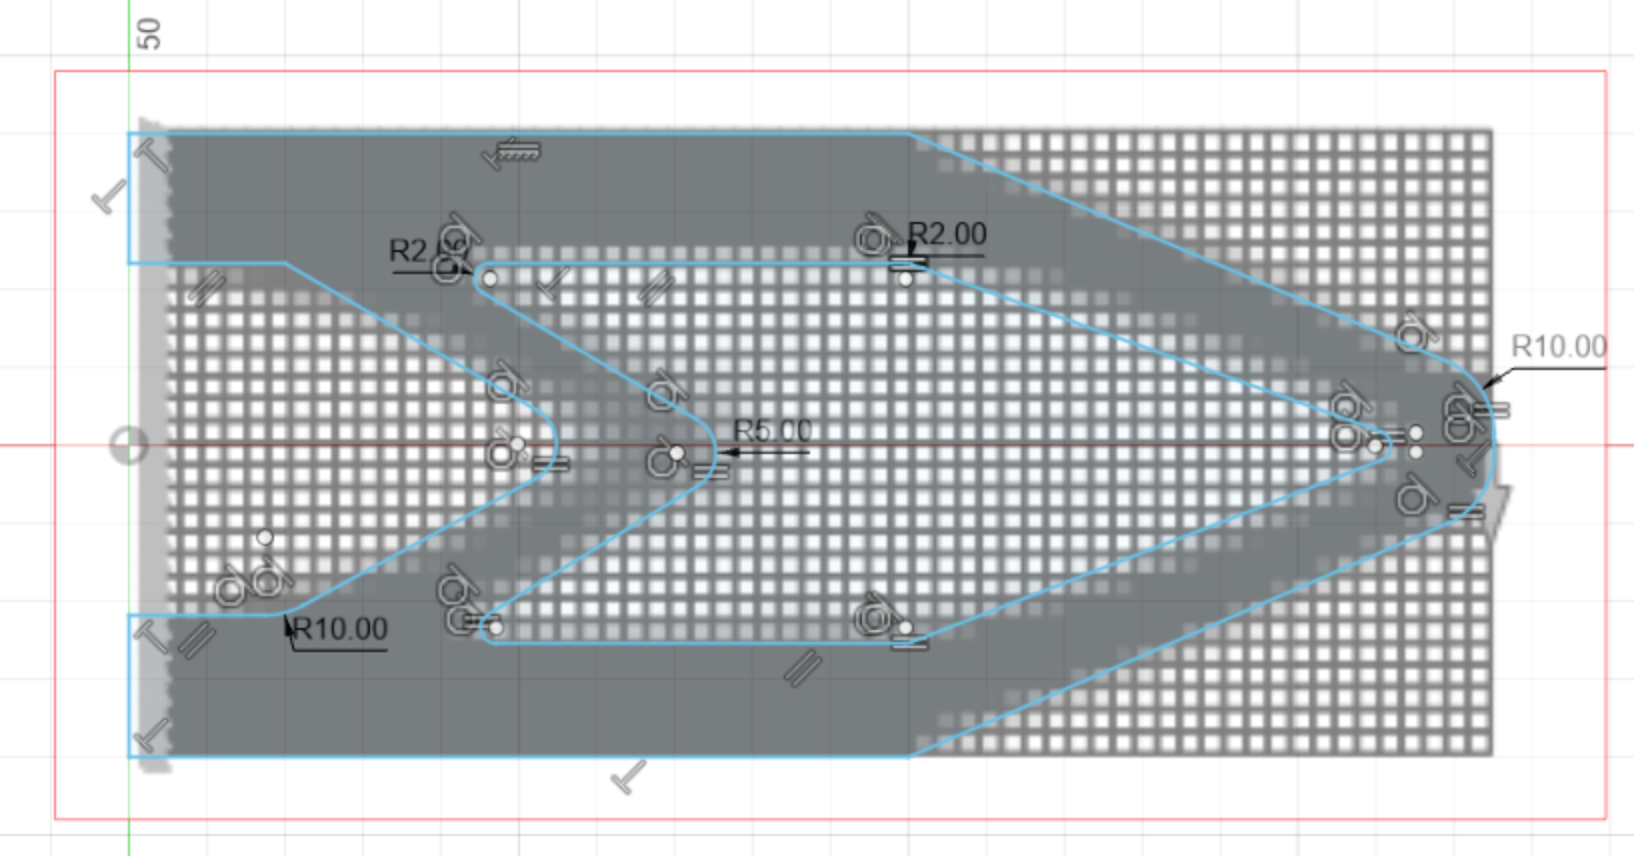
\includegraphics[width=0.7\linewidth]{figures/cantilever_template.png}
%     \end{center}
    
%     This is an interpretation of the cantilever beam as a sheet metal design:
%     \begin{center}
%         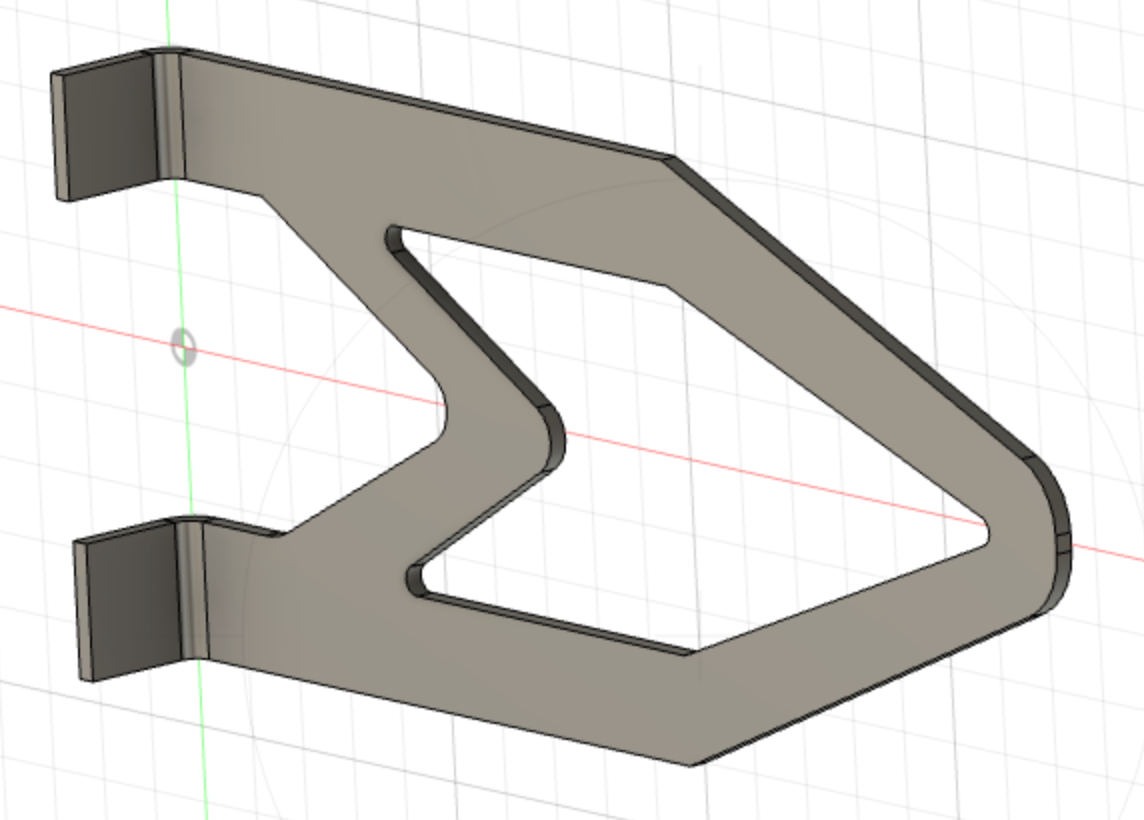
\includegraphics[width=0.7\linewidth]{figures/cantilever_design.png}
%     \end{center}
% \end{example}

\section{Shape optimization}
Shape optimization of continua seeks the optimal shape of the outer perimeter of a structure without adjusting the topology, i.e. without adding new perimeters like holes. The shape optimization problem for minimum compliance for a given volume constraint can be formulated analogously to trusses (see Equation \eqref{eq:shape_optimization}) as 

\begin{equation}
    \begin{aligned}
        \min_{\mathbf{x}} \quad & C(\mathbf{x}) = \mathbf{f} \cdot \mathbf{u}(\mathbf{x})\\
        \textrm{s.t.} \quad & g(\mathbf{x}) = \mathbf{d} \cdot \mathbf{A}(\mathbf{x}) - V_0 \le 0  \\
                            & \mathbf{x} \in \mathcal{X}
    \end{aligned}
    \label{eq:shape_optimization_continuum}
\end{equation}

A natural choice for design variables are the coordinates of nodes bounding the meshed domain, just as it has been done for trusses. However, this leads to jagged meshes with inaccurate stress calculations and limited deformation capabilities, as illustrated in the following example.

\begin{example}{Direct shape optimization of a cantilever beam}{directshapeexample}   
    Consider the cantilever beam from previous examples. If we choose nodal coordinates of the lower edge as design variables (highlighted with black dots) and try to minimize the compliance with a volume constraint, the stiffness improves slightly. However, the mesh is very irregular and leads to inaccurate stress calculations. Furthermore, the deformation is limited as it should neither result in collapsed elements nor highly stretched elements. 
    \begin{center}
        \includesvg[width=0.9\linewidth]{figures/cantilever_fem_naive_shape.svg}
    \end{center}
\end{example}

We may prevent the disadvantages of the direct nodal optimization by describing the deformation of the domain by a linear combination of basic shape modifications. This could be achieved by describing the perimeter with a spline representation \cite{Christensen2008} or by morphing operations on the mesh. Here, we decide to morph the mesh using radial basis functions \cite{Biancolini20}. 
A radial basis function (RBF) $\varphi \in \mathcal{R}$ is a function, that depends on the Euclidean distance $r = \lVert \mathbf{x}-\hat{\mathbf{x}} \rVert$ to some fixed point $\hat{\mathbf{x}}$.
We can use radial basis functions to interpolate the deformation of the mesh for a set of given control points $\hat{\mathbf{x}}_i$ as 
\begin{equation}
    \delta(\mathbf{x}) = \sum_{l=1}^P \gamma_i \varphi(\lVert \mathbf{x}-\hat{\mathbf{x}}_i \rVert).
\end{equation}

\begin{example}{Radial basis functions}{radialbasisexample}   
    Examples for radial basis functions are
    \begin{center}
        \begin{tabular}{ll}
            Gaussian: & $\varphi(r) = e^{-(\epsilon r)^2}$ \\
            Linear: & $\varphi(r) = r$ \\
            % Wendland C2: & $\varphi(r) = (1-\frac{r}{r_s})^4(4\frac{r}{r_s}+1),\quad  r \le r_s$ 
        \end{tabular}
    \end{center}
\end{example}

The interpolation should coincide with prescribed deformations at the control points $\delta_i$, i.e. 
\begin{equation}
    \delta(\mathbf{x}_i) = \delta_i \quad \forall i \in [1, P]
\end{equation}
must hold. To find weights fulfilling this condition, we can solve the linear system of equations 
\begin{equation}
    \mathbf{M} \cdot \pmb{\gamma} = \pmb{\delta} 
\end{equation}
with the interpolation matrix 
\begin{equation}
    M_{ij} = \varphi(\lVert \mathbf{x}_i-\hat{\mathbf{x}}_j \rVert) \quad i,j \in [1, P]. 
\end{equation}
Using the control points as design variables, we can modify the shape smoothly with a linear combination of basic shape modifications. The type of RBF constraints the solution space of shapes that can be achieved by shape optimization. 

\begin{example}{Shape modification with RBFs}{rbfshapeexample}   
    Consider the cantilever beam from previous examples. We can define a set of shape modifications with control points and Gaussian RBFs. Each shape modification is defined by its own design variable. 
    
    \begin{minipage}{.5\textwidth}
        \centering
        \includesvg[width=0.9\linewidth]{figures/cantilever_fem_shape_0.svg}
    \end{minipage}%
    \begin{minipage}{.5\textwidth}
        \centering
        \includesvg[width=0.9\linewidth]{figures/cantilever_fem_shape_1.svg}
    \end{minipage}
    \begin{minipage}{.5\textwidth}
        \centering
        \includesvg[width=0.9\linewidth]{figures/cantilever_fem_shape_2.svg}
    \end{minipage}%
    \begin{minipage}{.5\textwidth}
        \centering
        \includesvg[width=0.9\linewidth]{figures/cantilever_fem_shape_3.svg}
    \end{minipage}
    We may also use linear RBFs to define shape modifications:
    
    \begin{minipage}{.5\textwidth}
        \centering
        \includesvg[width=0.9\linewidth]{figures/cantilever_fem_shape_0_linear.svg}
    \end{minipage}%
    \begin{minipage}{.5\textwidth}
        \centering
        \includesvg[width=0.9\linewidth]{figures/cantilever_fem_shape_1_linear.svg}
    \end{minipage}
    \begin{minipage}{.5\textwidth}
        \centering
        \includesvg[width=0.9\linewidth]{figures/cantilever_fem_shape_2_linear.svg}
    \end{minipage}%
    \begin{minipage}{.5\textwidth}
        \centering
        \includesvg[width=0.9\linewidth]{figures/cantilever_fem_shape_3_linear.svg}
    \end{minipage}
\end{example}

We may reformulate the optimization problem now in terms of the design variables $\delta_i$ as 
\begin{equation}
    \begin{aligned}
        \min_{\pmb{\delta}} \quad & C(\pmb{\delta}) = \mathbf{f} \cdot \mathbf{u}(\pmb{\delta})\\
        \textrm{s.t.} \quad & g(\pmb{\delta}) = \mathbf{d} \cdot \mathbf{A}(\pmb{\delta}) - V_0 \le 0  \\
                            & \pmb{\delta} \in \mathcal{D}
    \end{aligned}
    \label{eq:shape_optimization_morph}
\end{equation}

Just like in shape optimization of trusses, target function and constraint function are generally non-linear and non-separable. Hence, we use MMA to approximate the problem and solve it equivalent to Equations \eqref{eq:shape_lagrangian} to \eqref{eq:shape_dual_solution}. We do not elaborate the analytical derivation of the gradients (this can be found e.g. in Chapter 6.3.2.2 in \cite{Christensen2008}), but simply rely on automatic differentiation to compute $\frac{\partial C}{\partial \delta_i}$ and $\frac{\partial g}{\partial \delta_i}$.


\begin{example}{Shape optimization of a cantilever beam}{cantilevershapeoptimizationexample}
    Consider the truss with Gaussian shape modifications from the previous example. We select the vertical degree of freedom of the five control points at the lower edge as design variables $\pmb{\delta} \in \mathcal{R}^5$.

    We want to solve for the optimal shape $\pmb{\delta}^*$ that minimizes the compliance of the structure without exceeding the initial volume of the truss. Hence, we formulate the following algorithm to solve the approximated problem: 
    \begin{enumerate}
        \item Define the cantilever FEM model with all nodes $\mathcal{N}$, elements $\mathcal{E}$, material properties $(E, \nu)$ , volume constraint $V_0$, design limits $\pmb{\delta}^l, \pmb{\delta}^u$ and the initial design choice $\pmb{\delta}^0$.
        \item Compute the mesh morphing weights given the current design $\pmb{\delta}^k$ according to
        \begin{equation}
             \pmb{\gamma}^k = \mathbf{M}^{-1} \cdot \pmb{\delta}^k 
        \end{equation}
        and morph the mesh with 
        \begin{equation}
            \delta(\mathbf{x}) = \sum_{l=1}^P \gamma_i^k \varphi(\lVert \mathbf{x}-\hat{\mathbf{x}}_i \rVert).
        \end{equation}
        \item Compute the displacements $\mathbf{u}^k$ by solving the FEM system for the morphed mesh.
        \item Compute the asymptotes as $\mathbf{L}^k = \pmb{\delta}^k - s (\pmb{\delta}^u - \pmb{\delta}^l)$ and $\mathbf{U}^k =\pmb{\delta}^k + s (\pmb{\delta}^u - \pmb{\delta}^l)$ with $s \in (0,1)$ during the first two iterations. In the following iterations, compute the lower asymptotes according to 
        \begin{equation}
            L^k_i = 
            \begin{cases}
                \delta^k_i - s  (\delta^{k-1}_i-L^{k-1}_i) & (\delta_i^k-\delta_i^{k-1})(\delta_i^{k-1}-\delta_i^{k-2}) < 0\\
                \delta^k_i - \frac{1}{\sqrt{s}}  (\delta^{k-1}_i-L^{k-1}_i) & \text{else}
            \end{cases}
        \end{equation}
        and the upper asymptotes according to 
        \begin{equation}
            U^k_i = 
            \begin{cases}
                \delta^k_i - s  (U^{k-1}_i-\delta^{k-1}_i) & (\delta_i^k-\delta_i^{k-1})(\delta_i^{k-1}-\delta_i^{k-2}) < 0\\
                \delta^k_i - \frac{1}{\sqrt{s}}  (U^{k-1}_i-\delta^{k-1}_i) & \text{else}
            \end{cases}
        \end{equation}
        \item Compute the move limits as 
        \begin{align}
            \tilde{\pmb{\delta}}^{l,k} &= \max(\pmb{\delta}^l,  0.9 \mathbf{L}^k + 0.1 \pmb{\delta}^k) \\
            \tilde{\pmb{\delta}}^{u,k} &= \min(\pmb{\delta}^u,  0.9 \mathbf{U}^k + 0.1 \pmb{\delta}^k)
        \end{align}

        \item Evaluate the gradients of the objective function $\frac{\partial C}{\partial \delta_i}$ and the constraint $\frac{\partial g}{\partial \delta_i}$ at $\pmb{\delta}^k$ using automatic differentiation. 

        \item Evaluate the analytical solution
            \begin{align}
                \hat{\delta}_i(\mu) &= 
                \begin{cases}
                    \delta^l_i 
                        &\textrm{if} \quad \frac{\partial C}{\partial \delta_i} > 0, \frac{\partial g}{\partial \delta_i} > 0 \\
                    \frac{U_i^k\omega + L_i^k}{1+\omega}, \quad \omega = \sqrt{-\mu\frac{(\delta_i^k-L_i^k)^2\frac{\partial g}{\partial \delta_i}}{(U_i^k-\delta_i^k)^2\frac{\partial C}{\partial \delta_i}}}
                        &\textrm{if} \quad \frac{\partial C}{\partial \delta_i}  > 0, \frac{\partial g}{\partial \delta_i} <0\\
                    \frac{U_i^k-L_i^k\omega}{1+\omega}, \quad \omega = \sqrt{-\mu\frac{(U_i^k-\delta_i^k)^2\frac{\partial g}{\partial \delta_i}}{(\delta_i^k-L_i^k)^2\frac{\partial C}{\partial \delta_i}}} 
                        &\textrm{if} \quad \frac{\partial C}{\partial \delta_i} < 0, \frac{\partial g}{\partial \delta_i}  > 0\\
                    \delta^u_i 
                        &\textrm{if} \quad \frac{\partial C}{\partial \delta_i}< 0, \frac{\partial g}{\partial \delta_i} < 0.
                \end{cases} \\
                \pmb{\delta}^* (\mu) &= \max\left(\tilde{\pmb{\delta}}^{l,k}, \min \left(\hat{\pmb{\delta}}(\mu), \tilde{\pmb{\delta}}^{u,k} \right)\right)
            \end{align}
        \item Perform a line search to find the maximum in 
            \begin{equation}
                \max_{\mu>0} \underline{\mathcal{L}}(\mu)
            \end{equation}
            with a gradient decent method. Once again, we may use automatic differentiation to compute the gradient for the optimization.
        \item Repeat with steps 2-8 until convergence or a maximum number of iterations is reached.
    \end{enumerate}
    
    The following figures show the evolution of the design variables during the optimization (left) and the final optimized structure (right) following this procedure. 

    \begin{minipage}{.5\textwidth}
        \centering
        \includesvg[width=0.9\linewidth]{figures/cantilever_fem_shape_variables.svg}
    \end{minipage}%
    \begin{minipage}{.5\textwidth}
        \centering
        \includesvg[width=0.9\linewidth]{figures/cantilever_fem_shape.svg}
    \end{minipage}
       
\end{example}


\bibliographystyle{unsrtnat}
\bibliography{literature} 